\subsection{2026-09-21 --- EDA round 2: what actually makes this problem hard}
\label{sec:eda-round-2}

Round 1 (Section~\ref{sec:eda}) characterised the data. This round targets the structure of the
prediction problem itself, to motivate features and architecture. Full notebook:
\texttt{src/EDA/eda\_round2.ipynb}. Twelve findings; the first four change how we should think
about the task.

\subsubsection*{The labels are not self-consistent.}
Cases are daily rolling, so consecutive cases overlap on 144 identical wall-clock hours (case
$N$'s hour $24{+}h$ is the same real timestamp as case $N{+}1$'s hour $h$), solved by SHOP from
essentially the same physical state.

\begin{figure}[htbp]
  \centering
  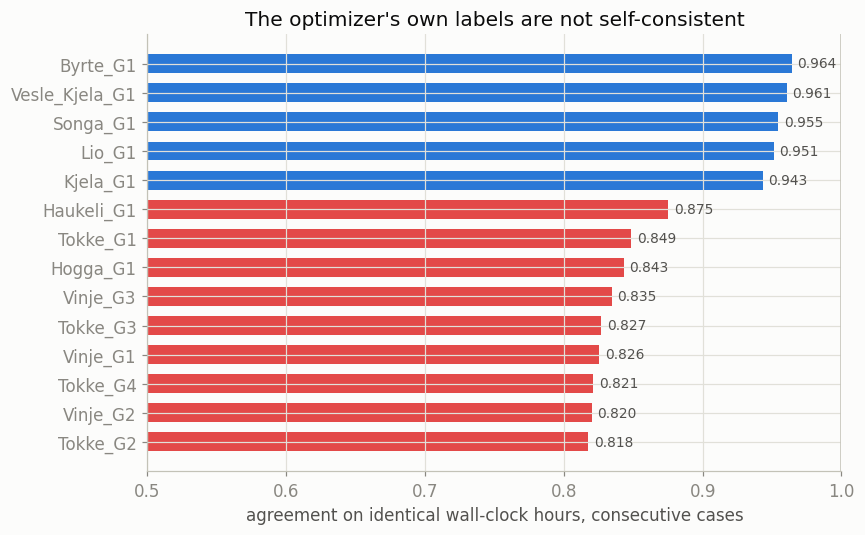
\includegraphics[width=0.72\linewidth]{figures/eda2_01_label_self_agreement.png}
  \caption{Agreement between consecutive cases on identical wall-clock hours.}
  \label{fig:eda2-agreement}
\end{figure}

\finding{\textbf{(1)} The same physical hour, re-solved one day later under a different 168-hour
horizon, gets a \emph{different} commitment decision \textbf{12\% of the time overall, and
$\sim$18\% for the Tokke and Vinje units} (Figure~\ref{fig:eda2-agreement}). This is not
measurement noise --- it is the optimizer reacting to end-of-horizon boundary conditions that a
wall-clock-indexed model cannot observe. It is an effective ceiling on achievable accuracy.}
\supersededby{sec:eda-round-3}{the ``effective ceiling'' inference is withdrawn --- the 12\% measurement stands, but it does not bound AUC.}

\begin{figure}[htbp]
  \centering
  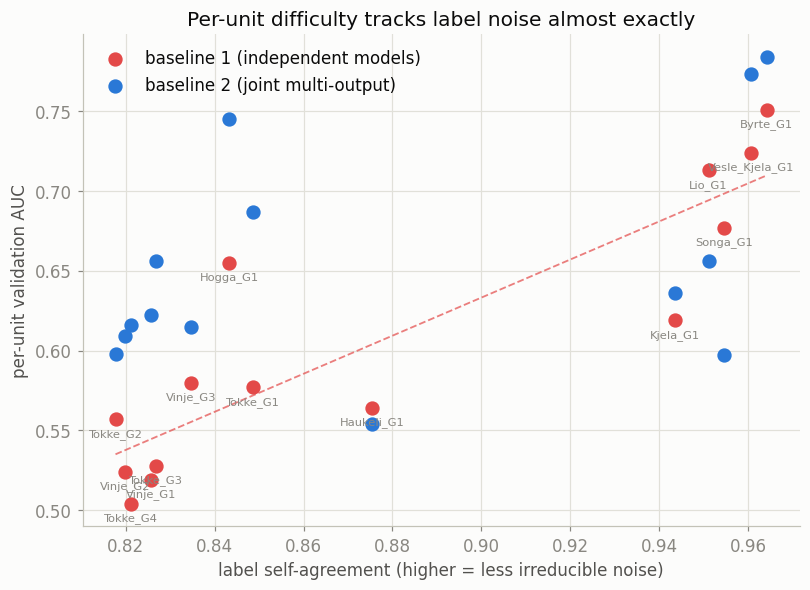
\includegraphics[width=0.72\linewidth]{figures/eda2_02_noise_vs_auc.png}
  \caption{Per-unit label self-agreement vs.\ per-unit validation AUC, both baselines.}
  \label{fig:eda2-noise-auc}
\end{figure}

\finding{\textbf{(2)} Label self-agreement correlates \textbf{$r=0.88$} with baseline-1 per-unit
AUC --- about \textbf{78\% of the variance in per-unit difficulty is explained by label noise
alone}, not by our features (Figure~\ref{fig:eda2-noise-auc}). The correlation drops to $0.42$
for the joint multi-output model, which is precisely the mechanism behind
Section~\ref{sec:multioutput}: pooling let the noisy Tokke/Vinje units borrow signal from their
correlated neighbours. It also finally explains the Songa\_G1 / Lio\_G1 regression left open in
Section~\ref{sec:capacity} --- those are the \emph{cleanest} units (95--96\% self-agreement),
and joint modelling pooled them with seven much noisier ones.}

\subsubsection*{The units inside a plant are identical, and strictly merit-ordered.}

\begin{figure}[htbp]
  \centering
  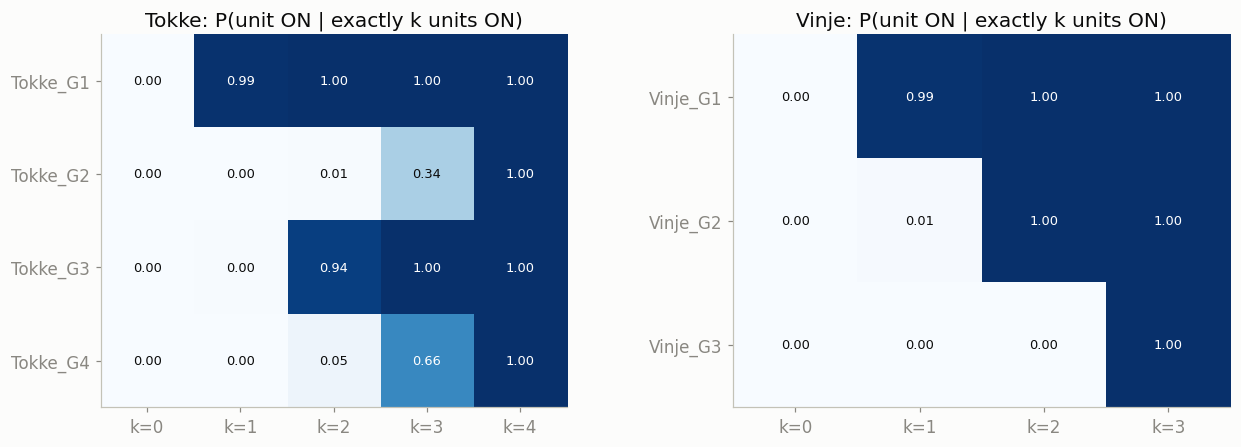
\includegraphics[width=0.95\linewidth]{figures/eda2_03_merit_order.png}
  \caption{$P(\text{unit ON} \mid \text{exactly } k \text{ units ON at the plant})$.}
  \label{fig:eda2-merit}
\end{figure}

\finding{\textbf{(3)} Every generator within a plant is \emph{physically identical} (Tokke:
4$\times$ $p_{\max}=107.5$\,MW; Vinje: 3$\times$ $p_{\max}=100$\,MW --- from the topology YAML we
had not been using). Commitment follows a near-strict merit order
(Figure~\ref{fig:eda2-merit}): Vinje is G1 $\to$ G1+G2 $\to$ all; Tokke is G1 $\to$ G1+G3 $\to$
then G4 or G2. \textbf{Knowing only how many units are on at a plant predicts exactly which ones
with 97.8\% (Tokke) and 99.9\% (Vinje) accuracy.}}

\finding{\textbf{(4)} Because the machines are interchangeable, \emph{which} identical unit takes
the marginal slot is partly an arbitrary solver tie-break --- this is the mechanism behind
finding (1). The only genuinely ambiguous slot is Tokke's third (G2 vs.\ G4, 34/66).}
\supersededby{sec:feature-themes}{penstock sharing explains the G1$\to$G3 ordering --- part of what looked arbitrary is hydraulic structure.}

\medskip
\noindent\textbf{Design implication.} The 14-output problem is really a small number of
\emph{per-plant count} problems plus a near-deterministic lookup. Predicting counts --- ordinal,
and far less noisy --- then expanding via merit order is a better-posed target than 14
individually-noisy binaries. This is the strongest architectural lead we have.

\subsubsection*{Remaining findings.}

\begin{figure}[htbp]
  \centering
  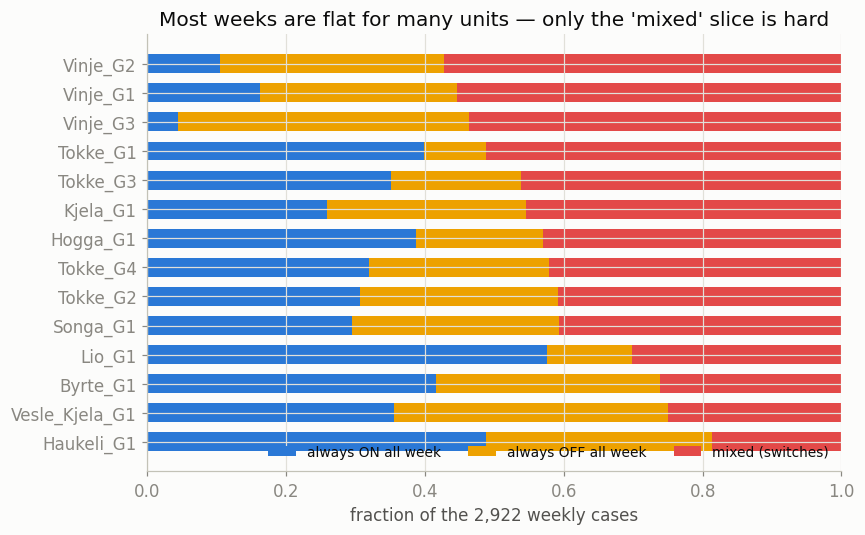
\includegraphics[width=0.72\linewidth]{figures/eda2_04_flat_vs_mixed.png}
  \caption{Share of weekly cases that are flat (never switch) vs.\ mixed, per unit.}
  \label{fig:eda2-flat}
\end{figure}

\finding{\textbf{(5)} Many weeks are completely flat: Haukeli\_G1 never switches in \textbf{81\%}
of weeks, Vesle\_Kjela\_G1 in 75\%, Byrte\_G1 in 74\% (Figure~\ref{fig:eda2-flat}). Only the
``mixed'' slice is genuinely hard, which suggests splitting ``does this unit move at all this
week?'' from ``when does it move?''.}

\begin{figure}[htbp]
  \centering
  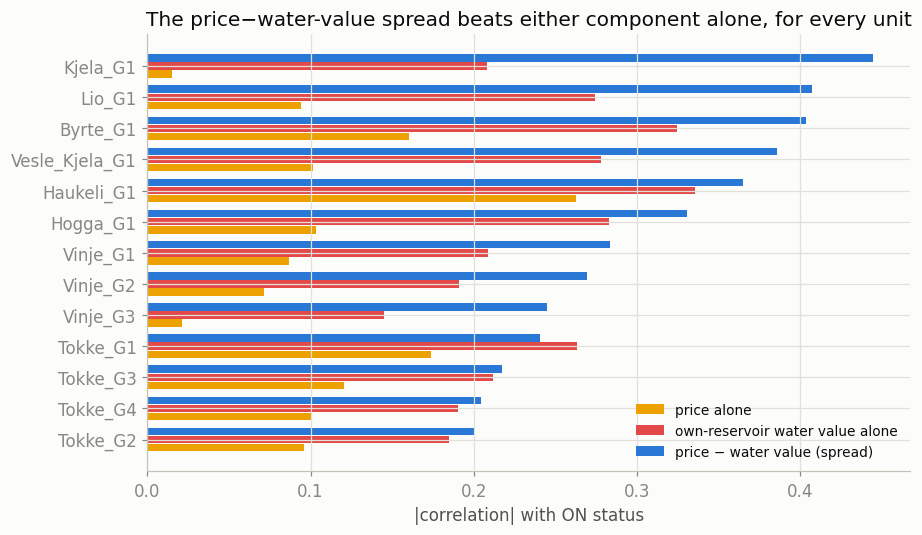
\includegraphics[width=0.78\linewidth]{figures/eda2_05_spread_vs_components.png}
  \caption{$|$correlation$|$ with ON status: price, own-reservoir water value, and their spread.}
  \label{fig:eda2-spread}
\end{figure}

\finding{\textbf{(6)} \texttt{storage\_Vatjern} and \texttt{storage\_Hyljelihyl} are
\textbf{literally constant} --- zero information. (The dataset PDF notes both reservoirs lack
historical records and were assumed 50\% full.) Drop them.}

\finding{\textbf{(7)} The \textbf{price $-$ own-reservoir water value spread} correlates more
strongly with ON status than either component alone, \emph{for every mapped unit}
(Figure~\ref{fig:eda2-spread}) --- the classic hydropower ``sell now vs.\ store it'' signal, and
the clearest single feature-engineering win available. Not currently in the feature set.}

\finding{\textbf{(8, a correction).} Normalising storage by each reservoir's \texttt{max\_vol} ---
proposed earlier in discussion as an important miss --- is a \textbf{no-op for tree models}: it is
a monotonic per-feature rescale, and trees are invariant to those. The 2462$\times$ spread in
reservoir size only matters for features that \emph{combine} reservoirs (e.g.\ system-wide
percent-full), or for linear/neural models. Recorded so we don't ``fix'' a non-problem.}

\begin{figure}[htbp]
  \centering
  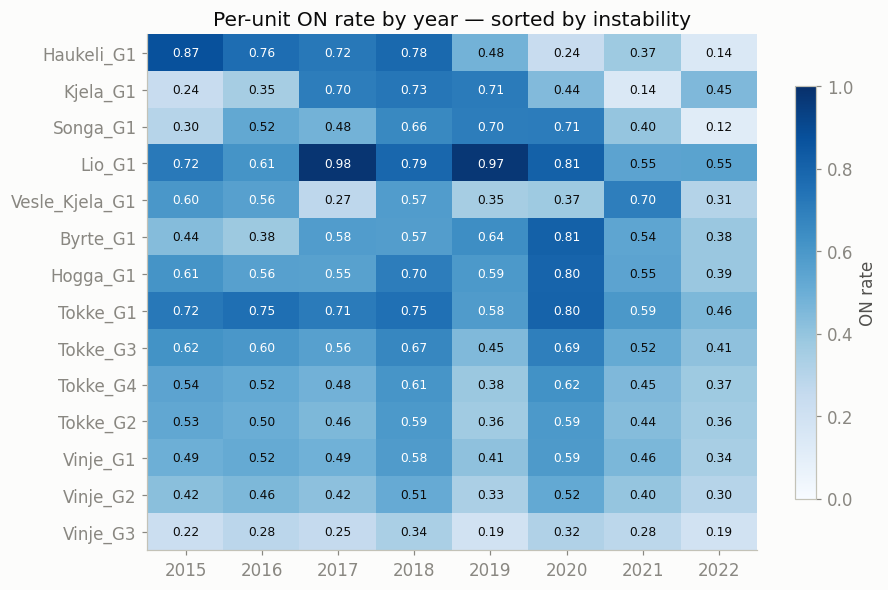
\includegraphics[width=0.78\linewidth]{figures/eda2_06_yearly_instability.png}
  \caption{Per-unit ON rate by year, sorted by instability.}
  \label{fig:eda2-yearly}
\end{figure}

\finding{\textbf{(9)} Severe per-unit non-stationarity: \textbf{Haukeli\_G1 collapses from 0.87
(2015) to 0.14 (2022)}; Songa\_G1 swings $0.30 \to 0.71 \to 0.12$
(Figure~\ref{fig:eda2-yearly}). These are structural changes in plant operation, not noise, and a
\emph{stronger} effect than the 2022 price spike flagged in Section~\ref{sec:eda}. Argues for
recency weighting or a shorter, more recent training window.}

\finding{\textbf{(10)} \texttt{min\_volume} constraints bind for exactly three reservoirs and only
in \textbf{July--October} --- a clean seasonal regime flag.}

\finding{\textbf{(11, a second correction).} \texttt{min\_flow} is \emph{always} active ($>0$ in
100\% of hours) for five of six rivers, so the binary ``is constrained'' flag suggested earlier
would be another constant column. The usable signal is the constraint's \textbf{level} and its
changes, not its existence.}

\finding{\textbf{(12)} The unit $\to$ reservoir map needs \textbf{multi-hop traversal}: Songa has
no direct reservoir edge at all, drawing from Songavatn and Bitdalsvatn through two tunnels and
discharging into Totak. Topology-derived features must walk the graph, not read single-hop edges.}
